\usepackage[utf8]{inputenc}
\usepackage{graphicx}
\usepackage{listings}
\usepackage{amsmath}
\usepackage{amssymb}
\usepackage{ae,aecompl}
\usepackage{fix-cm}
\usepackage{hyperref}

\usetheme{Goettingen}
\beamertemplatenavigationsymbolsempty
\beamertemplatetextbibitems
\setbeamertemplate{footline}[frame number]

\newcommand{\leftexp}[2]{{\vphantom{#2}}^{#1}{#2}}

\title{On the splitting problem of orbifolds via D-symbols}
\author{Boróczki, Lajos}
\date{June 24-28, 2013}

\begin{document}

\begin{frame}
  \maketitle
\end{frame}

\begin{frame}
  \mode<presentation>{\frametitle{Outline}}
  \tableofcontents
\end{frame}
\newpage

\section{D-symbols}
\begin{frame}
  \frametitle{D-symbol, an algebraic way to describe tilings}
  \begin{itemize}
    \item Based on the baricentric subdivision of a tiling
    \item Structure:
      \begin{itemize}
	\item D-diagram: $(dim+1)$ colored graph, which represents adjacencies of
	  simplex-orbits
	\item Matrix function on simplex orbits, which represents the number of
	  simpleces (not orbits) around a $(dim-2)$-dimensional edge
      \end{itemize}
    \item Constraints:
      \begin{itemize}
	\item Compatibility between the diagram and the matrix function
	\item Compatibility with baricentric subdivision
	\item Lower dimensional constraints
      \end{itemize}
    \item Every "nice" tiling has a corresponding D-symbol which is unambigous
      up to permutation \mode<article>{"Nice" tilings are the ones, whose
      baricentric subdivision has finitely many simplex-orbits and does not have
      ideal simplex-vertices except for 0-center or 3-center vertices.}
  \end{itemize}
\end{frame}

\subsection{Example}
\begin{frame}
  One of the simplest tilings of space $\mathbb{E}^3$ is with a square prism.
  It's baricentric subdivision and D-diagram: \mode<article>{figure \ref{abra:hasab_bari}.
  As adjacency relations are defined for every simplex orbit, we can skip
  showing the loops which map the orbits mirroring to a plane.}
  \begin{figure}
    \mode<article>{\caption{\label{abra:hasab_bari} Red:1, blue:2, green:3}}
    \center
    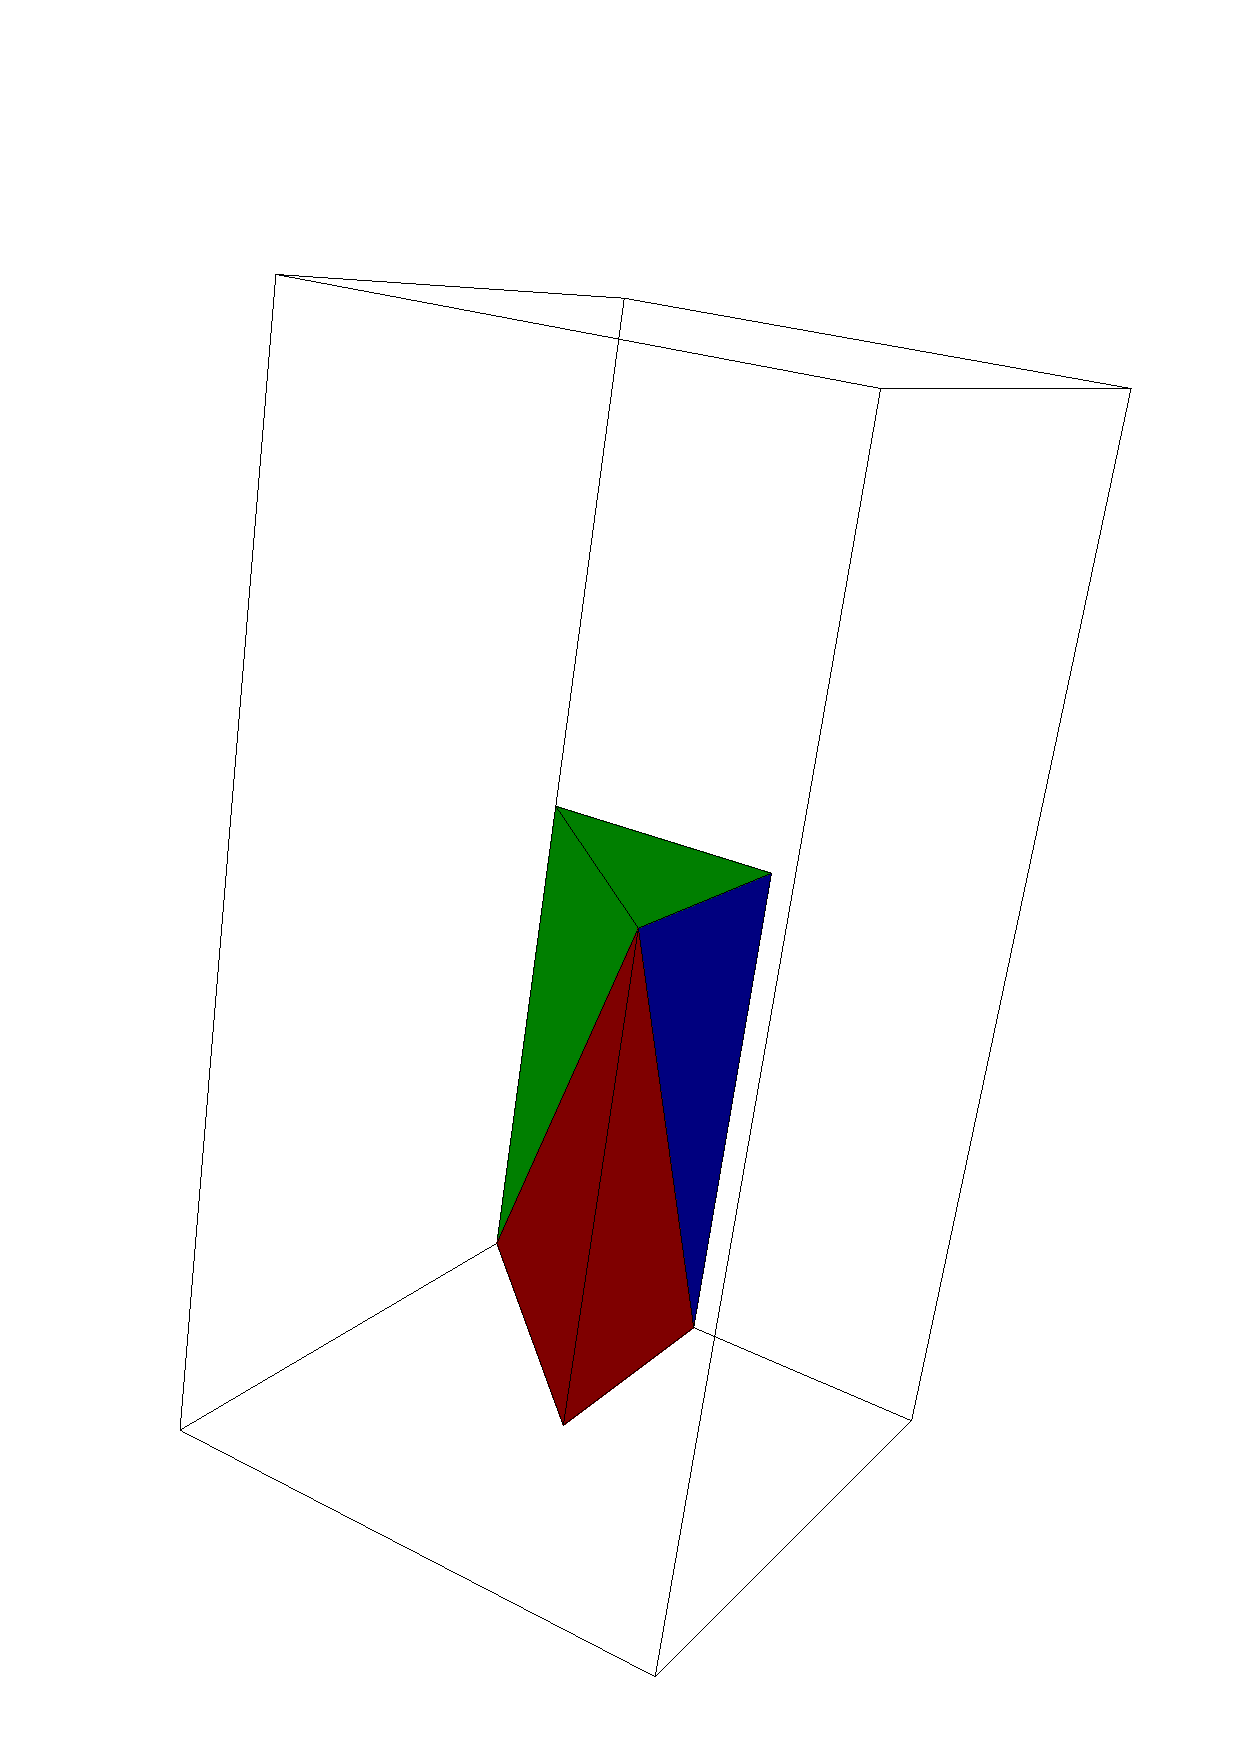
\includegraphics[width=0.4\textwidth]{hasab_bari.pdf}
    \includegraphics[width=0.35\textwidth]{hasab_D-graf.pdf}
  \end{figure}
  Notation:\\<all>
  \setlength{\unitlength}{1cm}
  $\sigma_0$:
  \begin{picture}(1,0.2)
    \multiput(0,0.1)(0.2,0){5}{\circle*{0.001}}
  \end{picture},
  $\sigma_1$:
  \begin{picture}(1,0.2)                                                                                 
    \multiput(0,0.1)(0.25,0){4}{\line(1,0){0.15}}                                                        
  \end{picture},
  $\sigma_2$:
  \begin{picture}(1,0.2)
    \put(0,0.1){\line(1,0){1}}
  \end{picture},
  $\sigma_3$:
  \begin{picture}(1.5,0.2)
    \multiput(0,0.1)(0.5,0){3}{\line(1,0){0.2}}
    \multiput(0.35,0.1)(0.5,0){3}{\circle*{0.001}}
  \end{picture}
\end{frame}

\mode<article>{
\begin{frame}
  $\mathcal{R}$ and $\mathcal{M}$ matrix-functions (where $\mathcal{D}$ is the set
  of simplex-orbits, $D_i\in\mathcal{D}$):
  \begin{equation*}
    \mathcal{R}(D_1)=
    \left(
    \begin{array}{cccc}
      1 & 1 & 2 & 1\\
      1 & 1 & 3 & 1\\
      2 & 3 & 1 & 2\\
      1 & 1 & 2 & 1
    \end{array}
    \right)
  \end{equation*}
  \begin{equation*}
    \mathcal{R}(D_2)=
    \left(
    \begin{array}{cccc}
      1 & 2 & 2 & 1\\
      2 & 1 & 3 & 2\\
      2 & 3 & 1 & 2\\
      1 & 2 & 2 & 1
    \end{array}
    \right)
  \end{equation*}
  \begin{equation*}
    \mathcal{R}(D_3)=
    \left(
    \begin{array}{cccc}
      1 & 2 & 1 & 1\\
      2 & 1 & 3 & 2\\
      1 & 3 & 1 & 1\\
      1 & 2 & 1 & 1
    \end{array}
    \right)
  \end{equation*}

  \begin{equation*}
    \forall D_i\in\mathcal{D}:\;
    \mathcal{M}(D_i)=
    \left(
    \begin{array}{cccc}
      1 & 4 & 2 & 2\\
      4 & 1 & 3 & 2\\
      2 & 3 & 1 & 4\\
      2 & 2 & 4 & 1
    \end{array}
    \right)
  \end{equation*}
\end{frame}
}

\section{Constraints for D-symbols}
The following constraints are needed for a D-symbol to have a corresponding
tiling.

\subsection{General constraints}
\begin{frame}
  D-symbol: $(\Sigma_I,\mathcal{D},\mathcal{M})$ triplets. \mode<article>{Where
  $I$ is the index set of the dimension ($|I|=dim+1$), $\Sigma_I$ is the set of
  adjacency operations (interpreted accordingly on the simplex-orbits and the
  simpleces), $\mathcal{D}$ is the set of simplex-orbits and $\mathcal{M}$ is
  the matrix-function on simpleces. These are the Delone-Delaney-Dress symbols,
  briefly D-symbols.}
  \begin{itemize}
    \item Natural constraints for D-diagrams:
      \begin{enumerate}
	\item $\mathcal{D}$ is finite
	\item Adjacency operations on simplex-orbits are involutive 
	  permutations\mode<article>{, this means $\forall i\in I, \sigma_i\in
	  \Sigma_I, \forall D\in \mathcal{D}$:
	  \begin{align*}
	    \sigma_i\sigma_i(D)=D 
	  \end{align*}
	  The degree of the uniformly colored edges in every vertice of the
	  diagram is $1$ or $2$. It is $2$ iff the edge is a loop.}
	\item Using not neighbouring operation-pairs we get back to the starting
	  vertice in at most $2$ steps\mode<article>{. \newline $\forall
	  i,j\in I, \forall D\in \mathcal{D}$:
	  \begin{align*}
	    |i-j|\geq 2 \Rightarrow (\sigma_j\sigma_i)^2(D)=D
	  \end{align*}}
      \end{enumerate}
    \item We can calculate the $\mathcal{R}$ matrix function\mode<article>{,
      which is the same for simplex-orbits as the $\mathcal{M}$ matrix function
      for simpleces: \newline $\forall i,j\in I, \forall D\in \mathcal{D}$:
      \begin{align*}
	r_{ij}(D)=r_{ji}(D)=\mathrm{min}\left\{r\in \mathbb{N}^+|(\sigma_j\sigma_i)^r(D)=D\right\}
      \end{align*}
      Constraints of the D-diagram on $\mathcal{R}$ matrix-function:
      $r_{ii}(D)=1$, and $|i-j|\geq 2 \Rightarrow r_{ij}(D)\leq2$}
    \item Constraints of the $\mathcal{M}$ matrix function:
      \begin{enumerate}
	\item Every element of $\mathcal{R}$ has to divide the appropriate
	  element of $\mathcal{M}$ (parameters)\mode<article>{. Because we have to get to the
	  same simplex walking around a $(d-2)$-dimensional face (which is an edge
	  in $3$ dimensions,) which means we have to get to the same
	  simplex-orbit too. The quotient of the elements of $\mathcal{M}$ and
	  $\mathcal{R}$ shows the periodicity of the tiling around the
	  $(d-2)$-dimensional face.
	  \newline $\forall i,j\in I, \forall D\in \mathcal{D}$:
	  $r_{ij}(D)|m_{ij}(D)$
	  }
	\item Orbits of adjacency-operation pairs\mode<article>{. An orbit can
	  be defined for every operation-pair and starting simplex-orbit
	  (diagram-vertex). Elements of $\mathcal{M}$ has to be the same inside
	  such an orbit. The reversed orbit has to contain the same number of
	  simpleces, so the matrices of $\mathcal{M}$ has to be symmetric.
	  \begin{align*}
	    &\forall i,j\in I, \forall D\in \mathcal{D} \\
	    &\mathcal{D}'=\left\{(\sigma_j\sigma_i)^k(D)|k\in
	    \mathbb{N}\right\}\cup\left\{\sigma_i(\sigma_j\sigma_i)^k(D)|k\in
	    \mathbb{N}\right\}\\
	    &\forall D_1,D_2 \in \mathcal{D}'\\
	    &m_{ij}(D_1)=m_{ij}(D_2)=m_{ji}(D_1)=m_{ji}(D_2)
	  \end{align*}
	  }
	\item The values of the main diagonal has to be $1$\mode<article>{,
	  because we have adjacency operations.}
	\item The values of the first diagonal above and below the main has to
	  be $\geq3$\mode<article>{. In case of nice tilings in 3 dimensions
	  every vertex joins at least 3 edges and 3 facets, every facet has at
	  least 3 edges and every edge joins 3 facets and 3 bodies.}
	\item Every other value has to be exactly $2$\mode<article>{, so we stay
	  compatible with baricentric subdivision.}
	  $\forall i,j\in I, \forall D\in \mathcal{D}$:
	  \begin{align*}
	    i=j & \Rightarrow m_{ij}(D)=1 \\
	    |i-j| = 1 &\Rightarrow m_{ij}(D)\geq3 \\
	    |i-j|\geq2 &\Rightarrow m_{ij}(D)=2
	  \end{align*}
      \end{enumerate}
  \end{itemize}
\end{frame}



\subsection{D-subsymbols}
\begin{frame}
  From now on we only consider $3$-dimensional D-symbols. \newline
  D-subsymbol:
  \begin{itemize}
    \item The $i$th D-subsymbols 
      $(\leftexp{c}{\Sigma_I}^i,\leftexp{c}{\mathcal{D}}^i,\leftexp{c}{\mathcal{M}}^i)$\mode<article>{ can be got by
      eliminating the $i$th operation from the diagram and the rows and columns
      of the matrix functions. ($c\in\mathcal{C}_i$ denotes the component.)}
    \item We can calculate the combinatorial curvature function of the subsymbol:
      \begin{align*}
	K(\leftexp{c}{\mathcal{D}}^i)=\sum_{D\in
	\leftexp{c}{\mathcal{D}}^i}\left(-1+\sum_{\substack{0\le j<k\le d \\
	j,k\ne i}}\frac{1}{m_{jk}(D)}\right)
	\begin{array}{cccc}
	  > & & S^2 \\
	  = & 0 & \mathbb{E}^2 \\
	  < & & H^2
	\end{array}
      \end{align*}
      \mode<article>{Based on the above formula one can decide, in which
      $2$-dimensional constant curvature space realizes the tiling.}
  \end{itemize}
  \mode<presentation>{\begin{minipage}[t]{0.45\textwidth}}
    \begin{itemize}
      \item Good orbifold criteria\mode<article>{: In the above mentioned
	spherical tiling case, we have to exclude bad orbifolds. The following
	options are excluded (given by both Convay's and Macbeath's notations):
	\begin{align*}
	  u=(+,0;[u];\{\}), & & 1<u;\\
	  *u=(+,0;[];\{(u)\}), & & 1<u;\\
	  uv=(+,0;[u,v];\{\}), & & 1<u<v;\\
	  *uv=(+,0;[];\{(u,v)\}), & & 1<u<v.
	\end{align*}}
      \item Visualization:
	\mode<article>{The subsymbol corresponds to the $(3-1)$-dimensional
	tiling around the $i$-indexed vertice-class indicated by the
	original D-symbol. So we have to get a spherical tiling around a real
	simplex-vertice (see Fig. \ref{fig:spherical_ex}), or a Euclidean tiling
	around an ideal simplex-vertex in the original tiling. We should not get
	hyperbolic tilings around a simplex-vertex, because this would mean an
	out-of-model vertex.}
    \end{itemize}
  \mode<presentation>{\end{minipage}
  \begin{minipage}[t]{0.5\textwidth}}
    \begin{figure}
      \mode<article>{\caption{\label{fig:spherical_ex}Spherical tiling around
      a simplex-vertex}}
      \center
      \includegraphics[height=2.5cm]{d3c3_2_vertice.pdf}
    \end{figure}
  \mode<presentation>{\end{minipage}}
\end{frame}

\begin{frame}
  Further constraints in $3$-dimensional D-symbols based on $2$-dimensional
  subsymbols (for every component):
  \begin{enumerate}
    \item For
      $(\leftexp{c}{\Sigma_I}^1,\leftexp{c}{\mathcal{D}}^1,\leftexp{c}{\mathcal{M}}^1)$ and
      $(\leftexp{c}{\Sigma_I}^2,\leftexp{c}{\mathcal{D}}^2,\leftexp{c}{\mathcal{M}}^2)$ the combinatorial curvature
      function has to be positive and the tiling has to be good
      orbifold\mode<article>{. Edge- and face-centered simplex-vertices has to
      be real vertices, so the tiling around them has to be an $S^2$ tiling.}
    \item For
      $(\leftexp{c}{\Sigma_I}^0,\leftexp{c}{\mathcal{D}}^0,\leftexp{c}{\mathcal{M}}^0)$ and
      $(\leftexp{c}{\Sigma_I}^3,\leftexp{c}{\mathcal{D}}^3,\leftexp{c}{\mathcal{M}}^3)$ the combinatorial curvature 
      function has to be non-negative, and if positive the tiling has to be good
      orbifold\mode<article>{. Vertex- and body-centered simplex-vertices can be
      real or ideal vertices, so the tiling around them can be an $S^2$ or an
      $\mathbb{E}^2$ tiling. (We do not exclude ideal body-centers because of
      the duality.)}
  \end{enumerate}
  These constraints lead to an upper bound of the parameters \mode<article>{as a
  system.}
\end{frame}

\section{Enumerating edge-transitive D-symbols}
\begin{frame}
  How can we use the D-symbols for $3$-dimensional edge-transitive tilings?
  \begin{itemize}
    \item Very simple new constraint: $|\mathcal{C}_1|=1$. The
      D-diagram cannot "fall apart" if we cancel it's $1$-colored (dashed)
      edges
    \item Enumerating diagrams becomes easier: Let's enumerate diagrams without
      $1$-colored edges, and put back them in every possible (good) way
    \item It can be proved that the maximal cardinality of such tilings is $24$
      based on the combinatorial curvature function of
      $(\leftexp{1}{\Sigma_I}^1,\leftexp{1}{\mathcal{D}}^1,\leftexp{1}{\mathcal{M}}^1)$.
      We could enumerate all of them. \mode<article>{Last time maximum: $18$.}
  \end{itemize}
\end{frame}


\section{Splitting}

\begin{frame}
  \frametitle{Splitting problem and the Thurston conjecture}
  Thurston conjecture:
  \begin{itemize}
    \item Every oriented prime closed 3-manifold can be cut along tori, so that
      the interior of each of the resulting manifolds has a geometric structure
      with finite volume.
    \item There are 8 possible geometric structures in 3 dimensions, which have
      at least one compact manifold modelled on itself: $S^3$, $E^3$,
      $H^3$, $S^2\times R$, $H^2\times R$, $\widetilde{SL2R}$, Sol,
      Nil.
  \end{itemize}
  Remarks:
  \begin{itemize}
    \item For non-orientable manifolds the "oriented double cover" method can be
      used\mode<article>{. Which maps manifold $M$ to $M\times Z/2Z$ with an
      appropriate pull-back operation. For example a Möbius-strip is mapped to a
      "double Möbius-strip" which is a ring.}
    \item In $2$ dimensions: every surface without boundary (2-manifold) has a
      geometric structure consisting of a metric with constant curvature
  \end{itemize}
\end{frame}

\begin{frame}
  \mode<article>{Using D-symbols one can examine the properties of orbifolds,
  but luckily the 3-manifolds in the conjecture are trivially orbifolds.}
  Finding splittings in a D-symbol:
  \begin{itemize}
    \item $S^2$-type splitting: Indicates a detail in the tiling, which is
      shrinkable to a single vertex\mode<article>{, so we get a similar tiling with
      less simplex-vertices, so with less simplex-orbits. (Possible bad
      orbifold problem.) (See fig. \ref{fig:s2splitting}.)}
      \begin{figure}
	\mode<article>{\caption{\label{fig:s2splitting} $S^2$-type splitting}}
	\center
	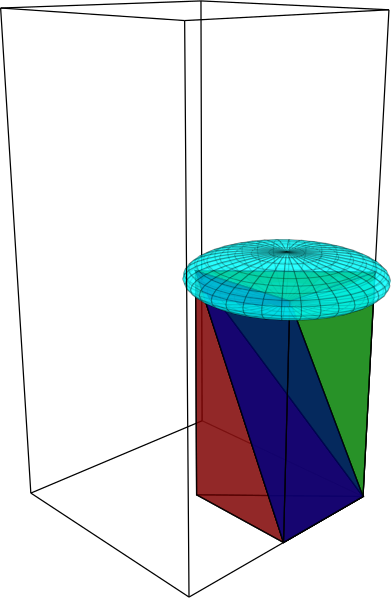
\includegraphics[height=2.5cm]{d3c3_2_splitting1.pdf}
      \end{figure}
    \item $E^2$-type splitting: In Thurston-conjecture "cut along tori". This
      indicates two parts in the tiling, in both parts the other part
      can be seen as an ideal vertex. \mode<article>{There are 2
      possible combinations, from which only the first one indicates a
      splitting, the second one indicates a fibration. (See fig.
      \ref{fig:e2splitting}.)}
      \begin{figure}
	\mode<article>{\caption{\label{fig:e2splitting} $E^2$-type splittings}}
	\center
	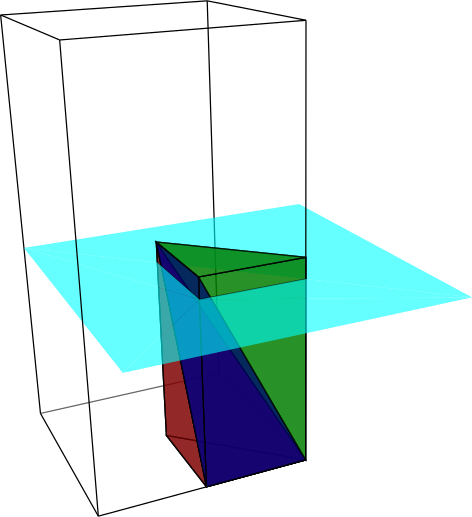
\includegraphics[height=2.5cm]{d3c3_2_splitting2_alt1.pdf}
	\hspace{0.1\textwidth}
	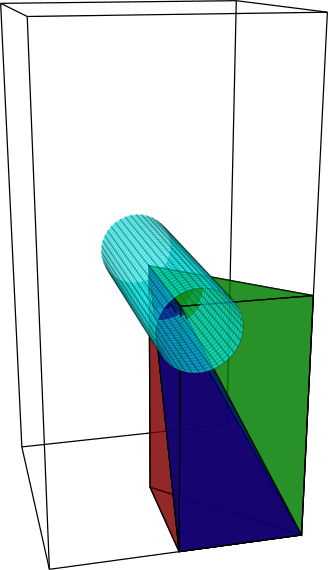
\includegraphics[height=2.5cm]{d3c3_2_splitting2_alt2.pdf}
      \end{figure}
  \end{itemize}
\end{frame}

\begin{frame}
  Further constraints for D-symbols without splittings
  \begin{itemize}
    \item Based on the $3$-dimensional D-diagram, we can describe the tiling's
      simplex-vertice classes and the edges between simplex-vertice classes.
      Take this system as a graph and examine the border between every possible
      2-partitions \mode<article>{(where both partitions have at least 2
      vertices) using the above mentioned combinatorial curvature function.}
    \item Every such border gives us a $2$-dimensional tiling of which we
      already know the generators and relations. \mode<article>{There's a slight
      problem though: these tilings can have triangles and quadrangles
      (splitting a tetrahedron can give you a triangle or a quadrangle,) but our
      combinatorial curvature function is for triangles only. This can be
      resolved quite easily by triangulating the quadrangles.}
    \item Examining such "splitting-candidates", we can get lower bounds
      for the parameters of D-symbols without splittings. \mode<article>{If and
      only if there is no splitting in a D-symbol, then every such 2 dimensional
      tiling is $H^2$-tiling and this is a lower bound for $m$-values in the
      combinatorial curvature function.}
    \item (If we could find one such that it's not realizable in any of the 8
      Thurston-geometries, then this would be a counter-example of the Thurston
      conjecture.)
  \end{itemize}
\end{frame}

\begin{frame}[plain]
  \frametitle{Illustration}
  \only<2>{\mode<presentation>{That looks like a screenshot, let's see the original at
  \href{http://math.bme.hu/~boroczki/D-symbols-edge-transitive/d3c6/31.html}{my
  homepage.} }}
  \mode<article>{Figure \ref{fig:d3c6_31}. looks like a screenshot, let's see
  the original at
  \href{http://math.bme.hu/~boroczki/D-symbols-edge-transitive/d3c6/31.html}{my
  homepage.}
  Constructing a visualisation of the fundamental
  domain for edge transitive tilings is pretty straightforward: Take the 1 or 2
  simplex edges between 0 and 1 vertices, and put around them the simpleces
  using their single parameter.}
  \begin{figure}
    \mode<article>{\caption{\label{fig:d3c6_31} 31st D-symbol with cardinality 6
    in 3D}}
    \center
    \includegraphics[height=0.5\textwidth]{d3c6_31.pdf}
    \hspace{0.1\textwidth}
    \includegraphics[width=0.3\textwidth]{d3c6_31_diag.pdf}
  \end{figure}
\end{frame}

\begin{frame}
  \nocite{DHM93,D87,Du88,H93,LM90,Ma67,M94,T82,VS93,F94,F03}
  \bibliographystyle{plain}
  \mode<presentation>{\fontsize{5pt}{0}}
  \bibliography{dsym}
\end{frame}

\begin{frame}
  \frametitle{Questions?}
  \center\large Questions?
\end{frame}

\end{document}
